% --*- coding:utf-8-unix mode:latex -*--
%\include{Begin}
%%%%%%%%%%%%%%%%%%%%%%%%%%%%%%%%%%%%%%%%%%%%%%%%%%%%%%%%%%%%%%%%%%%%%%%%%%%%%%%

\section{野外炊事}

\subsection{日時・場所}

\begin{tabular}{p{2zw}rp{38zw}}
  日時 & : & 2019年4月5日(金) 16:20 $\sim$ 19:00\\
  場所 & : & 野外炊事場
\end{tabular}

\subsection{目的}
新入生同士及び在学生,教職員が協力して料理を作ることにより,親睦や交流をはかるきっかけにしてもらう.

\subsection{タイムスケジュール}
% 時刻は必ず4桁(00:00)で書くこと!!!
\begin{longtable}{p{3zw}p{39zw}}
  16:20 & \textbf{◎ 野外炊事場到着}\\
        %& \ \  \textbullet \ \ \underline{野外炊事統括(高島)} \\
        %& \ \  - A棟で待機し,肉を渡す準備をする \\
        & \ \  \textbullet \ \ \underline{各班スタッフ} \\
        & \ \  - 各班のプラカードが置かれている机に誘導する \\
        & \ \  - 野外炊事場で点呼が完了したら小島に報告し,本部で道具・食材を受け取る \\
        & \ \  \underline{※雨天時:傘は邪魔にならない場所(机の下など)に置く} \\\\
  16:25 & \textbf{◎ アイスブレイキング} \\
        & \ \  \textbullet \ \ \underline{各班スタッフ} \\
        & \ \  - 班内の教職員,スタッフ,新入生で,自分の名前,呼んでほしいニックネーム,得意な料理,野外炊事の意気込みを言い合う(教職員のニックネームは割愛する) \\
        & \ \  - スタッフはこの意気込みから各自の力量を推測し,役割分担に役立てる \\
        & \ \  - 移動中に仲良くなったとスタッフが判断した場合は,アイスブレイキングを割愛してもよい \\\\

  16:30 & \textbf{◎ 調理開始(レシピ参照)} \\
        & \ \  \textbullet \ \ \underline{野外炊事統括(小島)} \\
        & \ \  - 班到着チェック後,道具・食材の配布を行う(人数に注意) \\
        %& \ \  - 肉配布の際,着火剤を1班4欠片渡す \\
        & \ \  - 全班チェック後は見回りをする \\
        & \ \  \textbullet \ \ \underline{各班スタッフ} \\
        & \ \  - 班内で役割分担を行い,調理を開始する \\
        & \ \  - 各班のスタッフは新入生が全員映るように調理風景を撮る(スマホでも可) \\
        & \ \  - 薪係は薪置き場に薪を,食器係は食器置き場に食器を取りに行く \\
        & \ \  - 調理が完了した班から食事をとる(食事開始前に班ごとで集合写真を撮る) \\
        & \ \  - 食事が終わり次第片付けをする \\
        & \ \  - 怪我をした場合は,報告slackに連絡し,小松から救急箱を受け取り対応する \\%(未変更)
        & \ \  - 各班,抜ける可能性がある人がいる班は2人構成,もしくは隣の班が2人構成になっているのでスタッフが抜ける場合には声をかけ,新入生だけの状態にしないようにする.\\

  18:00 & \textbf{◎ 片付け開始}\\
        & \ \  \textbullet \ \ \underline{女性教員のいる班の代表} \\
        & \ \  - 食事が終了する頃に,報告slackに連絡する \\
        & \ \  \textbullet \ \ \underline{角原} \\
        & \ \  - 女性教員がいる全ての班(4つ)から食事終了の連絡がきたら,それぞれの班の女性教職員に声をかけ,(就寝場所)に誘導する \\
        & \ \  - 誘導前に鍵係(小谷)から鍵をもらって,途中で第一・二研修室により,各自荷物を取る \\

        & \ \  \textbullet \ \ \underline{鍵係(小谷)} \\
        % \ \  - 食事終了の連絡がきたら,事務室へ移動し,第一集会室・第二研修室・指導者棟(慎太郎と龍馬)・つどいの広間の鍵を受け取る \\
        %& \ \  - その後,第一集会室の鍵を開け待機する \\

        & \ \  - 小谷は片付けが終わり次第,先に戻り,角原から鍵を受け取り第一・二研修室を開けて,帰ってきた新入生たちに荷物を渡す \\
        & \ \  - 教員紹介後見つかった忘れ物は,新入生が荷物を取りに来たとき,持ち主がいないか呼びかける \\

        & \ \  \textbullet \ \ \underline{野外炊事統括(小島)} \\
        & \ \  - 5班分の片付けが終了するころに内線30番で職員の方に連絡する \\
        & \ \  \textbullet \ \ \underline{各班スタッフ} \\
        & \ \  - 各班スタッフは片付けが終わった時に報告slackに連絡する \\
        & \ \  - ?未使用の薪は薪庫に,燃えかけの薪と灰はそれぞれ別の場所に捨てる \\
        & \ \  - 食器の汚れをチェックする \\
        & \ \  - 片付けが終わったら,職員の方を呼びに行き,チェックを受ける \\
        & \ \  - ?職員のチェック後,食器は食器置き場へ戻す \\
        & \ \  - ?コンテナは各班のスタッフが返却する \\
        & \ \  - 大学の備品は一箇所に集めて机の上に置いておく \\
        & \ \  - 用意した備品は一箇所に集めて机の上に置いておく \\\\


  18:45 & \textbf{◎ 片付けチェック}\\
        & \ \  \textbullet \ \ \underline{野外炊事統括:小島,西森} \\
        & \ \  - 片付け終了後,各班の終了点呼を行う \\
        & \ \  - 全班完了次第,野外炊事統括(小島)は最終チェックをする.(ゴミの回収,忘れ物チェック) \\
        & \ \  - 用意した備品は全班終了後に小島が回収する \\
        & \ \  - ?西森車へゴミを積み込みゴミ庫で処分後,本館へ移動する \\
        & \ \  \textbullet \ \ \underline{各班スタッフ} \\
        & \ \  - 片付けが終了し,職員のチェックを受けた班は,野外炊事統括(?小島)に直接報告する \\
        & \ \  - ?スタッフはコンテナを持ったまま班員を第一・二研修室に誘導し,各自荷物を取る \\
        %& \ \  - 入浴係(藤田,日下)は小谷から各指導者棟の鍵を受け取る \\
        & \ \  - ?その後,コンテナを食堂で返却し,班員をくろしお棟へ誘導する(暗いので携帯のライトアプリを使用する) \\
        & \ \  - 4班((丸田),小島の荷物を,1班((伊崎)は西森の荷物を第一研修室で回収し宿泊部屋に向かう \\
        & \ \  - 就寝場所への誘導終了後,報告slackに連絡する \\
        & \ \  \textbullet \ \ \underline{小谷} \\
        & \ \  - 第一・二研修室に忘れ物がないか確認後,自分の荷物を持って就寝場所に移動する \\
        & \ \  \underline{※雨天時:帰り道は十分に注意する} \\
        & \ \  \underline{※雨天時:傘を忘れない} \\\\

  19:00 & \textbf{◎ 終了(完全撤退)} \\\\
\end{longtable}

\subsection{人員配置}
\subsubsection{スタッフの役割}
\begin{itemize}
  \item 救急箱担当;小松
  \item 野外炊事統括:小島
  \item ?車運転:西森
  \item 各班担当:各班2名〜3名
  %\item 肉担当:高島(三浦,下出が肉を持ってくるので,その肉を置き場所を確認する)
  \item 片付け:西森,小島
  \item 鍵担当:小谷
  \item 女性教職員誘導:角原
\end{itemize}

\subsubsection{班の割り当て}
\begin{itemize}
 \item A棟 : 1班(伊崎,西森),2班(生野,貞松),3班(北村,小谷),4班(丸田,小島)
 \item B棟 : 5班(塩谷,立岩),6班(吉田,藤田),7班(青山,堀川),8班(高橋(龍),小松)
 \item C棟 : 9班(石野,日下),10班(別役,高橋(慎)),11班(角原,以西),12班(新田,宮尾)
 \item D棟 : 13班(東),14班(中島,横田),15班(新川,藤沢),16班(江川)
 \item E棟 : 17班(高島),18班(野田),19班(渡辺),20班(真壁,斎藤)
\end{itemize}

\subsubsection{班内の役割(目安)}

準備時
\begin{itemize}
  \item 薪係:2名
  \item 食器係:2名
\end{itemize}

調理時
\begin{itemize}
  \item 火をおこす係:1名
  \item カレー係:2名
  \item 米を炊く係:1名
  \item ?お茶を作る係:1名
  \item 皿を洗う係:1名
\end{itemize}

\subsubsection{野外炊事班}
\begin{figure}[H]
\begin{center}
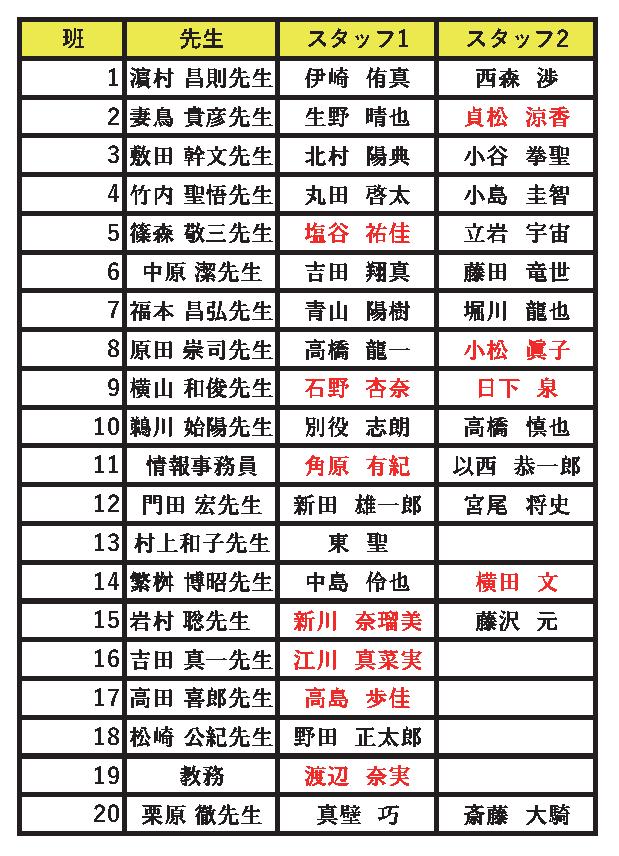
\includegraphics[scale=0.9]{./09/yagaisuijihanwake.eps}
\end{center}
\end{figure}


\subsection{必要物品(1班分)}
\begin{itemize}
  \item ピーラー:1個(20個)
  \item 野外炊事班のプラカード:20個
  \item ゴミ袋:2班で1つ(11個)
  \item 軍手:20組
  \item ふきん:3枚
  \item 新聞紙:20日分
  \item うちわ:1個
  \item チャッカマン:2個
  \item 着火剤:5個
  \item 食器用消毒液:10個
  \item ライトアプリ(足下を照らすアプリであれば指定なし)
  \item 救急箱(大学からかりる)
\end{itemize}

\subsection{全体配置(晴れ)}
\begin{figure}[h]
\begin{center}
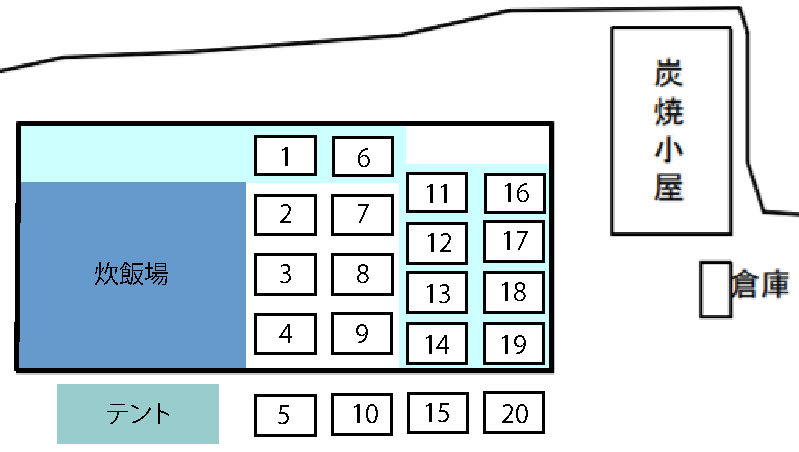
\includegraphics[width = 10cm]{./09/yagaisuiji.eps}
\end{center}
\end{figure}

\subsection{全体配置(雨)}
\begin{figure}[h]
\begin{center}
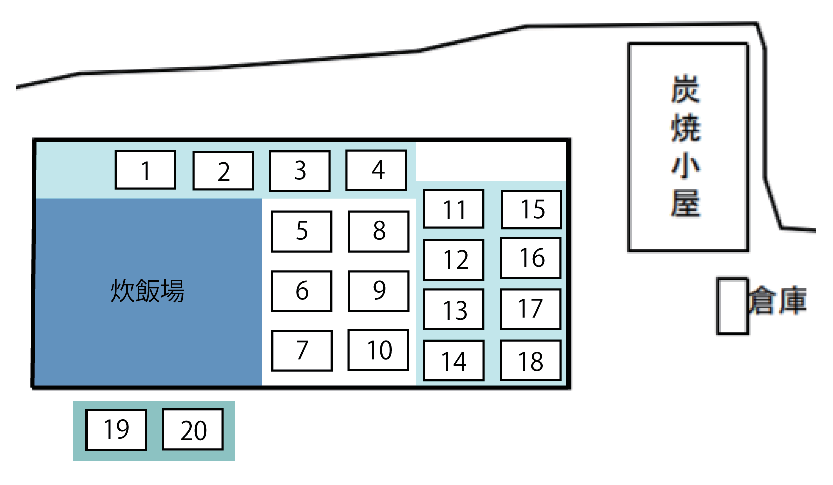
\includegraphics[width = 10cm]{./09/yagaisuijirain.eps}
\end{center}
\end{figure}


\subsection{注意事項}
\begin{itemize}
  \item 新入生が手持ち無沙汰にならないように,人数分配を最初から終わりまで出来るだけ決めておく
  \item 時間の確認(終了時間のデッドラインや各作業の目安を確認する)
  \item 食器の個数と食材の確認
  \item 怪我に注意(火の扱い,包丁等)
  \item 食器を洗う際は,確実に汚れを落とす(点検をスムーズに行うため)
  \item 統括,各班スタッフ,新入生との「報連相」を密に行う
  \item 鍵は担当が厳重に注意して管理する
\end{itemize}

\subsection{レシピ}
\begin{itembox}[l]{カレーのレシピ}
  \begin{enumerate}
    \item ピーラーでじゃがいも、にんじんの皮をむく
    \item 野菜は大きすぎると火が通らないので細かく薄く切る
    \item 肉は半分に切る
    \item お湯を沸かす(お茶用かつカレー非常時用に利用)
    \item 切った具材を鍋に入れ、ひたひたになるまで水を入れる(水を入れすぎない)
    \item 火にかける
    \item 沸騰まで放置する(フォーク等で刺し、じゃがいもやにんじんに穴があくかを確認する)
    \item ルーを開封前に細かく砕く
    \item 混ぜながらルーを入れる
    \item ルーが溶けたら終了
    \item カレーが濃いときはお茶用に沸かしているお湯で薄めると良い
  \end{enumerate}
\end{itembox}

\begin{itembox}[l]{ご飯のレシピ}
  \begin{enumerate}
    \item 米を研ぐ
    \item 米の表面から一差し指第2関節に行かないぐらいまで水を入れる
    \item 火にかける

    \item 最初は中火(底に火がふれるくらい)、途中で強火(はんごう全体が火に包まれるくらい)で加熱してやると美味しいご飯ができる
    \item 吹きこぼれて、吹きこぼれが乾いたら火から遠ざける(火にかけはじめて20分ほど待って吹きこぼれなかったらふたを開けて確認する)
    \item ご飯がべしゃべしゃの状態で炊けてしまったときはかまどの端っこの方(あまり火の当たらないところ)で1分ごとはんごうを回しながら水分を飛ばしてやると良い
  \end{enumerate}
※吹きこぼれている時には、絶対にふたは空けない
\end{itembox}

%\begin{itembox}[l]{お茶のレシピ}
%    \begin{enumerate}
%    \item やかんに水を入れて沸騰させる(カレーを薄めるためにお湯を使うかも知れないので早いうちからお茶っ葉を入れない)
%    \item 沸騰したらお茶っ葉をやかんに入れる
%    \item 10分ほど煮て火から遠ざける
%  \end{enumerate}
%※水を完全に沸騰させないと、味が不味くなる
%\end{itembox}

\subsection{備考}
\begin{itemize}
\item 基本的に各班代表者が報告slackへの連絡を行う
\item 火起こしの作業が遅れているときは他の班から人員を派遣する(火起こしが上手そうな人)
\item 燃え残りの薪と灰は捨てる場所が違うので注意する
\item ?片付けチェックで職員を呼ぶタイミングは、最初の5班から片付け終了の連絡を受けてから小島が内線30番に電話する
\item 進行状況は随時各班のスタッフが報告slackに連絡する(見回りにいけないとこもあるかもしれないので)
\item 宮尾は翌日の朝のつどいの旗揚げの新入生(男女1名ずつ)を野外炊事中にスカウトする(なるべく目立つ子を)
\end{itemize}


%%%%%%%%%%%%%%%%%%%%%%%%%%%%%%%%%%%%%%%%%%%%%%%%%%%%%%%%%%%%%%%%%%%%%%%%%%%%%%%
%\include{End}
